\section{Parallel Communication Interfaces}
\subsection{Vorteile paralleler Kommunikation}
\begin{compactitem}
    \item Parallele Kommunikation hat theoretischen Vorteil eines Durchsatzes, der N-mal grösser für eine N-Bit breite Kommunikation ist (gegenüber seriell).
    \item Parallele Kommunikation hat zusätzlichen Vorteil, dass keine Serialisierung / De-Serialisierung an Quelle und Senke benötigt wird $\rightarrow$ reduziert Hardwarekosten und Komplexität
\end{compactitem}

\subsection{Nachteile paralleler Kommunikation}
\begin{compactitem}
    \item In der Praxis stimmt die Aussage des Durchsatzes nicht. Clock und Data Skew bewirken, dass die Kommunikationsgeschwindigkeit der Geschwindigkeit des langsamsten Bits entspricht.
    \item Crosstalk zwischen den Leitungen ist ein weiteres Problem der parallelen Kommunikation. Parallele Datenleitungen beeinflussen sich gegenseitig und dadurch kann sich die Bitfehlerrate leicht erhöhen.
    \item Mit zunehmender Systemgröße von SoC-Komponenten hat die Anzahl der IOs ein Niveau erreicht, in dem die parallele Kommunikation mit der grossen Anzahl von benötigten IOs für die Off-Chip-Kommunikation mehr und mehr unwirtschaftlich wird $\rightarrow$ IOs verbrauchen Chipfläche und erzeugen somit Kosten.
\end{compactitem}

\subsection{AXI - Advanced eXtensible Interface}
Das AXI-Protokoll ist für eine hohe Bandbreite sowie eine kleine Latenzzeit ausgelegt. Es werden getrennte Lese- und Schreibbusse unterstützt. Weiter sind getrennte Busse für die Adressen sowie die Steuersignale vorhanden. Zusätzlich können auch sogenannte Burst-Transaktionen durchgeführt werden.

\subsubsection{Bustopologie und Modes}
Die AXI-Schnittstelle ist eine Multiple-Master-Multiple-Slave-Schnittstelle. Diese Topologie erfordert eine physikalische Verbindungsstruktur, die jeden Master mit jedem Slave verbindet. Die Topologie erlaubt es, dass zwei Master gleichzeitig Daten übertragen. Um Kollisionen zu vermeiden, ist ein Arbiter erforderlich, der entscheidet, welcher Master Zugriff auf einen Slave erhält. Es gibt verschiedene Verfahren, wie z. B. round-robin, preemptive priority, non-preemptive priority...
Der Lese- und Schreibkanal des Adressbusses kann geteilt werden, um Platz zu sparen. Dasselbe gilt auch für den Datenbus. Im AXI-Protokoll, müssen zwei Teile unterschieden werden:
\begin{compactitem}
  \item AXI interface ist eine 1-zu-1 Verbindung mit 5 unabhängigen Kanälen für Schreib-/Lesetransaktionen. Das AXI interface verbindet immer einen Master mit einer Slave-Node.
  \item AXI interconnect verbindet N Master mit N Slave Nodes. Es ist ein Logikblock, bestehend aus Arbitern, Multiplexern, Pipeline-Registern, vielen Verbindungen, einigen FIFOs und anderer Logik-Primitiven. AXI interconnect arbeitet als Switchbox um Signale von einer Master zu einer Slave-Node zu routen.
\end{compactitem}

\subsubsection{Kanäle}
\begin{multicols}{2}
    \begin{figure}[H]
     	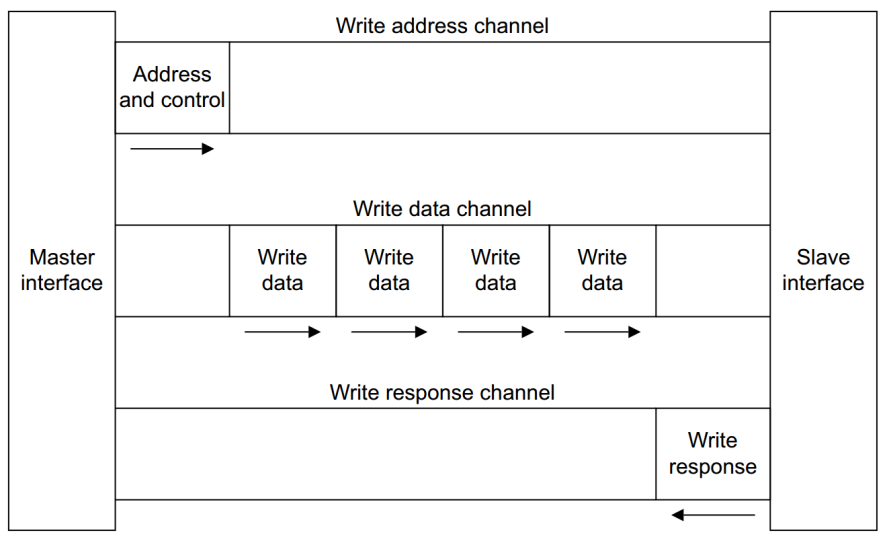
\includegraphics[width=0.4\textwidth]{images/AXI_Write_Data_Channels.png}
     \end{figure}
     \begin{figure}[H]
     	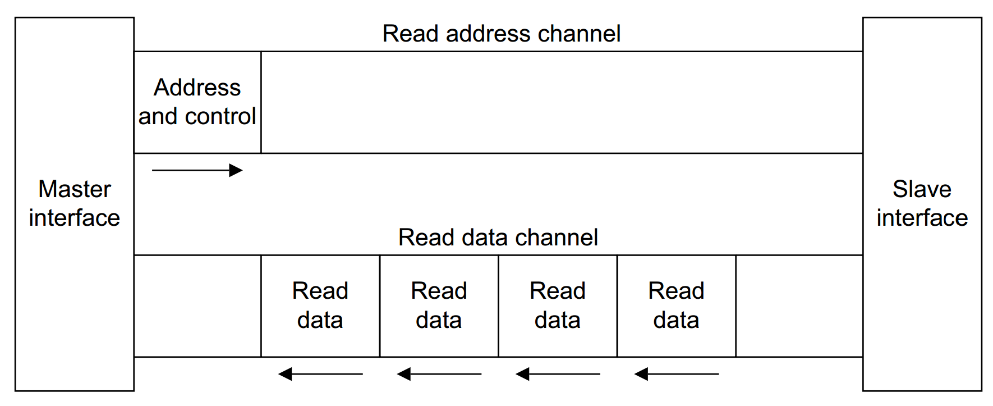
\includegraphics[width=0.5\textwidth]{images/AXI_Read_Data_Channels.png}
     \end{figure}
\end{multicols}
\begin{multicols}{2}
    \begin{compactitem}
        \item AW (write address channel) $\rightarrow$ Master zu Slave
        \item W (write data channel) $\rightarrow$ Master zu Slave
        \item WR (B) (write response channel) $\rightarrow$ Slave zu Master
        \item AR (read address channel) $\rightarrow$ Master zu Slave
        \item R (read data channel) $\rightarrow$ Slave zu Master
    \end{compactitem}
\end{multicols}

\begin{multicols}{2}
    \subsubsection{Handshaking}
    Für jeden Übertragungskanal existiert ein Handshaking. Ein Vorteil dieser Funktionsweise besteht darin, dass der Empfänger sowie der Sender die Geschwindigkeit der Datenübertragung steuern können.
     \begin{figure}[H]
     	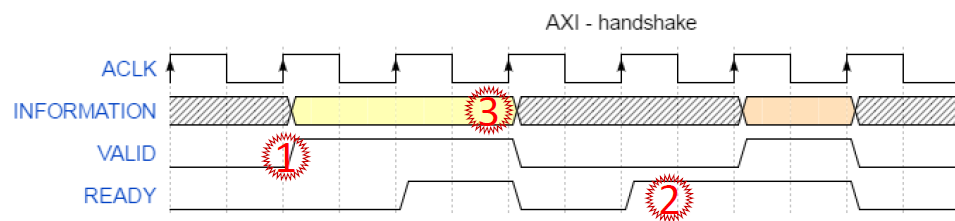
\includegraphics[width=0.5\textwidth]{images/AXI_Handshaking.png}
     \end{figure}
\end{multicols}
\begin{compactenum}
    \item Der Datensender setzt das Valid Signal, um anzuzeigen, dass Informationen verfügbar sind.
    \item Der Datenempfänger setzt das Ready Signal, um anzuzeigen, dass die Information akzeptiert werden kann.
    \item Eine Übertragung von Daten tritt auf, wenn sowohl das Valid als auch das Ready Signal an einer Taktflanke high sind.
\end{compactenum}

\begin{multicols}{2}
    \begin{figure}[H]
     	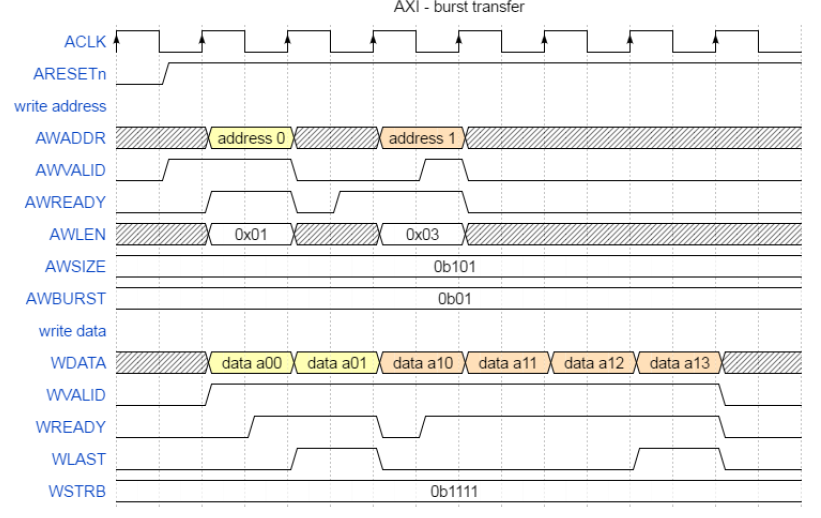
\includegraphics[width=0.5\textwidth]{images/AXI_Burst_Transfer.png}
     \end{figure}
    \paragraph{Burst Mode}
    Anstatt ein einziges Wort oder Byte in einer Transaktion zu senden, wird  im Burst-Modus ein gesamter Block von Daten gesendet. Dies ist sehr nützlich bei der Übertragung grosser Datenmengen.
\end{multicols}

\subsubsection{Varianten}
\begin{compactitem}
    \item AXI 4: Maximale Performance. Burst-Modus bis zu 256 Zyklen pro Adresse. Für Hochleistungsdatenaustausch.
    \item AXI-Lite: Vereinfachte Version von AXI 4. Für speicherabgebildete Einzeltransaktionen. Kein Burst. Für kleinen Datendurchsatz wie Austausch von Steuerungseinstellungen.
    \item AXI-Stream: Für High-Speed-Streaming. Keine Adressphase (nicht speicherzugeordnet). Unbegrenzte Datenburstgrösse. Daten vom Master zum Slave.
\end{compactitem}

\begin{multicols}{2}
\subsubsection{AXI Interconnect Block}
Für den Anschluss des AXI-Bussystems werden viele Interconnect Blöcke verwendet.
\begin{compactitem}
    \item Agiert als Slave vom PS
    \item Dient als Master für die Signalweiterleitung vom PS zu verschiedenen AXI-IP-Instanzen (Slaves).
    \item Unterstützt auch eine Protokollkonvertierung (z.b. Verbindung von AXI 3 und AXI 4)
\end{compactitem}
\vfill\null
\columnbreak
\begin{figure}[H]
  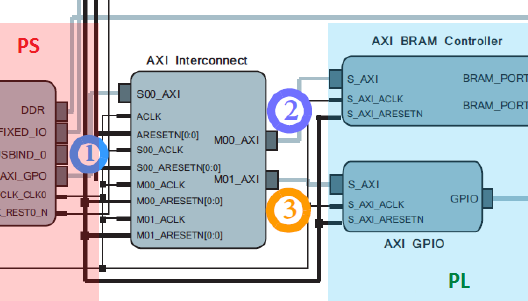
\includegraphics[width=0.5\textwidth]{images/AXI_Interconnect.png}
 \end{figure}
\end{multicols}
\begin{compactitem}
  \item SASD (Shared address bus and shared data buses) $\rightarrow$ Für weniger komplexe Systeme
  \item SAMD (Shared address bus and multiple data buses) $\rightarrow$ Durchsatz des Adressbusses ist kleiner als derjenige des Datenbusses, aufgrund der Burst-Fähigkeit des Datenkanals.
  \item MAMD (Multiple address bus and multiple data buses) $\rightarrow$ Für komplexe Systeme
\end{compactitem}

\subsubsection{Zynq: Processing System $\leftrightarrow$ Programmable Logic}
\begin{multicols}{2}
  Datenübertragung zwischen PS und PL erfolgt via AXI. Jede Schnittstelle realisiert einen kompletten AXI Bus. Insgesamt sind 9 AXI Schnittstellen vorhanden.
  \begin{figure}[H]
   	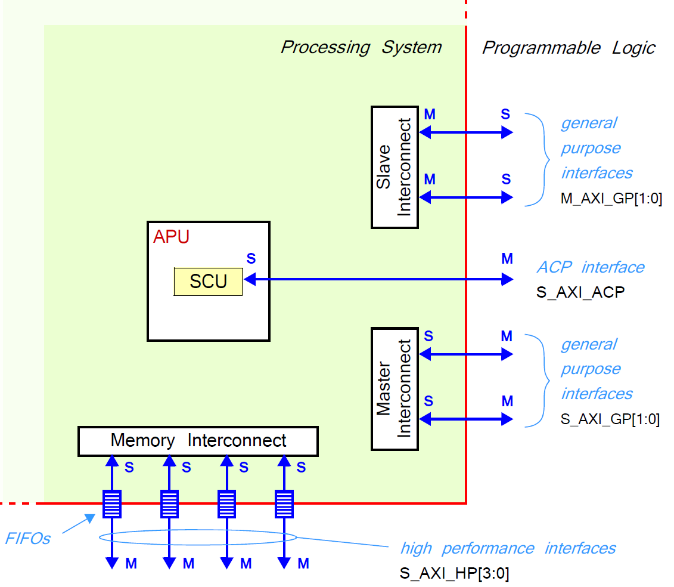
\includegraphics[width=0.5\textwidth]{images/AXI_PL_PS.png}
   \end{figure}
\end{multicols}
